\documentclass{article}

\usepackage[final,nonatbib]{neurips_2024}

\usepackage[utf8]{inputenc}
\usepackage[T1]{fontenc}
\usepackage{hyperref}
\usepackage{url}
\usepackage{booktabs}
\usepackage{amsfonts}
\usepackage{nicefrac}
\usepackage{microtype}
\usepackage{xcolor}
\usepackage{graphicx}
\usepackage{amsmath}
\usepackage{amssymb}
\usepackage{multirow}
\usepackage{subcaption}
\usepackage{tikz}
\usetikzlibrary{arrows.meta, positioning, shapes.geometric, calc}

\title{Hybrid Edge-Guided Diffusion Refinement for Leakage-Free Low-Dose CT Denoising}

\author{%
  Zhexi Feng \\
  Department of ECE \\
  University of California, San Diego \\
  \texttt{zhf023@ucsd.edu} \\
  \And
  Bingrui Zhang \\
  Department of ECE \\
  University of California, San Diego \\
  \texttt{biz005@ucsd.edu} \\
}

\newcommand{\method}{EG-LDM}
\newcommand{\hybrid}{Hybrid EG-LDM}

\begin{document}

\maketitle

\begin{abstract}
Low-dose CT denoising must suppress noise without inventing unsupported anatomy. We study this problem on raw LIDC-IDRI DICOM under a leakage-free patient-level protocol, and we refine our original edge-guided latent diffusion prototype into a \textbf{hybrid diffusion-refinement system}. The final model combines four ingredients: a strong RED-CNN pixel-fidelity anchor, a compact edge-guided latent diffusion module, 2.5D neighboring-slice conditioning, and auxiliary reconstruction losses that penalize both intensity and gradient error. At inference time, diffusion acts conservatively: it contributes a small correction to the RED-CNN anchor and is then re-grounded to the observed LDCT slice through edge-adaptive residual fusion. We curate 1{,}010 patients and 243{,}957 valid axial slices after CT-only filtering, duplicate SOP removal, and verified HU conversion, then synthesize paired low-dose observations with signal-dependent Gaussian corruption. On the real-anatomy test split, the standalone edge-guided \method{} reaches PSNR 28.46, SSIM 0.710, and RMSE 0.0765, improving over both raw LDCT and a no-edge diffusion ablation. The proposed \hybrid{} is substantially stronger, achieving PSNR 35.12, SSIM 0.9040, and RMSE 0.03558, slightly surpassing a matched RED-CNN baseline at 35.02, 0.9028, and 0.03598 under the same medium-scale protocol. The resulting picture is precise: diffusion is not yet strongest as a standalone denoiser in this setting, but explicit edge-guided diffusion refinement on top of a strong deterministic anchor yields the best overall fidelity while preserving a conservative, measurement-grounded reconstruction strategy.
\end{abstract}

\section{Introduction}
Computed Tomography (CT) is indispensable in screening, diagnosis, and longitudinal follow-up, but image quality remains tightly coupled to radiation dose. The long-standing clinical motivation for low-dose CT is clear: dose reduction lowers cumulative radiation exposure, yet also amplifies quantum noise and structured artifacts that interfere with subtle anatomy and low-contrast lesion visibility~\cite{brenner2007}. The resulting restoration problem is therefore not merely cosmetic. A useful method must improve fidelity while preserving structures that are already present in the underlying scan.

The difficulty is not only removing noise, but removing it conservatively. In natural-image restoration, a model may be rewarded for perceptually plausible detail synthesis. In CT, however, a plausible but unsupported edge can be more problematic than residual noise, because it changes the visual evidence available to a reader. This makes hallucination control, structural fidelity, and transparent evaluation protocol design central to the problem formulation rather than secondary engineering choices.

The LDCT literature has evolved from residual CNN denoisers such as RED-CNN~\cite{chen2017} to adversarial and structurally aware models~\cite{yang2018,yi2018,you2018}. These methods can be highly effective, but direct regression often tends toward over-smoothing, whereas adversarial training can emphasize texture realism without an equally explicit mechanism for structural control. Diffusion models~\cite{sohldickstein2015,ho2020,nichol2021,song2021sde,song2021ddim} offer a compelling alternative because they optimize a denoising trajectory instead of a single feed-forward mapping. Conditional diffusion has already proved effective for restoration-style problems in natural images~\cite{saharia2021}, latent diffusion~\cite{rombach2022} reduces the computational burden, and ControlNet~\cite{zhang2023controlnet} provides a natural way to inject spatial constraints. In medical inverse problems, score-based and diffusion priors have already shown strong promise in settings such as accelerated MRI~\cite{chung2022}.

This paper studies how far a structurally controlled diffusion model can be pushed on real CT anatomy once the benchmark is made credible and the model is allowed to collaborate with a strong deterministic restorer. Our focus is deliberately pragmatic. Rather than relying on slice-level random splits or synthetic anatomical phantoms, we build the study around raw LIDC-IDRI DICOM with persisted patient-level partitions and verified HU conversion~\cite{armato2011}. Rather than asking whether a small standalone diffusion prototype can dominate all baselines, we ask a sharper question: can edge-guided diffusion provide useful anatomical refinement on top of a strong pixel-fidelity backbone, and can that gain be demonstrated under a benchmark where data leakage and evaluation ambiguity have been removed? The main contributions of the work are:
\begin{itemize}
    \item A leakage-free patient-level LIDC-IDRI DICOM pipeline with CT-only filtering, duplicate-slice removal, HU verification, and persisted split/index artifacts.
    \item A hybrid denoising architecture that combines RED-CNN anchoring, edge-guided latent diffusion refinement, 2.5D neighboring-slice conditioning, auxiliary reconstruction losses, and conservative anchor-aware fusion at inference.
    \item A real-data comparison on curated LIDC-IDRI anatomy showing both that edge guidance improves the diffusion family over a no-edge ablation and that the final \hybrid{} slightly surpasses the standalone RED-CNN baseline under a matched medium-scale protocol.
\end{itemize}

\section{Related Work}
\textbf{CT denoising.}
Image denoising predates deep learning and includes a rich family of nonlearned priors and patch-based estimators such as non-local means and BM3D~\cite{buades2011,dabov2007}. Deep residual denoisers later translated these ideas into trainable feed-forward models, ranging from DnCNN~\cite{zhang2017dncnn} in natural-image denoising to paired medical-image restorers such as RED-CNN~\cite{chen2017}. Deep LDCT restoration has since been shaped by residual encoder-decoder architectures, U-Net-style backbones~\cite{ronneberger2015}, adversarial objectives, and explicitly structure-aware losses. Later works incorporated perceptual and adversarial supervision, including WGAN-VGG~\cite{yang2018}, sharpness-aware conditional GANs~\cite{yi2018}, and structurally sensitive multi-scale networks~\cite{you2018}. Collectively, these studies established both the strength of deterministic restoration and the central trade-off between aggressive denoising and structure preservation.

\textbf{Diffusion and controllable generation.}
Recent generative models replace direct prediction with iterative denoising. The original nonequilibrium formulation of diffusion models~\cite{sohldickstein2015}, DDPM~\cite{ho2020}, improved DDPM~\cite{nichol2021}, score-based stochastic differential equation models~\cite{song2021sde}, and DDIM~\cite{song2021ddim} define the modern diffusion toolkit. Restoration-oriented conditional diffusion has also been explored successfully in natural-image settings such as super-resolution~\cite{saharia2021}. Latent diffusion~\cite{rombach2022} reduces memory and runtime by moving generation to a compressed representation, and ControlNet~\cite{zhang2023controlnet} adds an effective conditioning interface through zero-initialized residual pathways, making it particularly appealing when one wants to enforce spatial cues without redesigning the full backbone.

\textbf{Medical-image motivation.}
Medical imaging benefits from diffusion priors when uncertainty and fidelity must be balanced carefully. Score-based reconstruction has already demonstrated encouraging behavior in MRI inverse problems~\cite{chung2022}. Our work transfers that broader motivation to CT denoising, with two practical differences: we use an explicit edge prior extracted from the noisy input itself, and we center the evaluation around patient-level leakage prevention, which is essential for a realistic restoration benchmark on volumetric medical data.

\section{Method}
\subsection{Problem Setup}
Let $x \in \mathbb{R}^{H \times W}$ denote a clean CT slice and let $y \in \mathbb{R}^{H \times W}$ denote its low-dose counterpart. In our benchmark, $x$ comes from real LIDC-IDRI DICOM after HU conversion and clipping, while $y$ is synthesized with signal-dependent Gaussian noise:
\begin{equation}
    y = x + \eta(x), \qquad \eta(x) \sim \mathcal{N}\!\left(0,\sigma(x)^2\right).
\end{equation}
The task is to estimate $\hat{x}$ from $y$ such that the restoration reduces noise while preserving anatomically meaningful boundaries.

The design is guided by three constraints. First, all conditioning signals must be derived from the noisy acquisition itself rather than from the target, so that the model does not receive oracle structure during either training or inference. Second, the system should remain conservative near strong boundaries, where unsupported hallucinated edges are clinically undesirable. Third, diffusion should not be forced to carry the full burden of pixel fidelity if a strong deterministic denoiser can already provide a reliable intensity anchor. These principles shape the hybrid architecture, the training objectives, and the final reconstruction rule.

\subsection{Hybrid Anchor-Conditioned Diffusion}
Our final model treats diffusion as a \emph{refinement module} around a strong pixel-fidelity baseline rather than as a standalone denoiser. Given a noisy slice $y$, we first obtain a deterministic anchor
\begin{equation}
    a = \mathcal{A}(y),
\end{equation}
where $\mathcal{A}$ is a pretrained RED-CNN~\cite{chen2017}. The anchor already removes most of the synthetic low-dose corruption and provides a high-quality intensity estimate. Diffusion is then tasked with making a smaller, anatomically guided correction around this anchor instead of reconstructing the entire image from scratch.

We keep a compact latent representation $z_0 = \mathcal{E}(x)$, where $\mathcal{E}$ is an identity-style autoencoder with downsampling factor $8$. A $256 \times 256$ slice becomes a $32 \times 32 \times 4$ latent tensor. This choice is pragmatic: under medium-scale training budgets, a weakly trained learned VAE can become the dominant source of blur, obscuring whether structural conditioning itself is useful. The identity-style latent bottleneck preserves the computational advantages of latent diffusion while avoiding a confounding autoencoding failure mode.

Diffusion training follows the standard noise-prediction objective~\cite{ho2020}. For timestep $t$ and Gaussian noise $\epsilon$,
\begin{equation}
    z_t = \sqrt{\bar{\alpha}_t} z_0 + \sqrt{1-\bar{\alpha}_t}\,\epsilon,
\end{equation}
and the denoiser $\epsilon_{\theta}$ predicts $\epsilon$ conditioned on four signals:
\begin{equation}
    \mathcal{C} = \{c_{\text{LDCT}}, c_{\text{ctx}}, c_{\text{anchor}}, c_{\text{edge}}\}.
\end{equation}
Here $c_{\text{LDCT}}$ is the latent encoding of the center noisy slice, $c_{\text{ctx}}$ is a 2.5D context token sequence from neighboring slices, $c_{\text{anchor}}$ is the latent encoding of the RED-CNN anchor, and $c_{\text{edge}}$ is a one-channel edge map. The base diffusion term is
\begin{equation}
    \mathcal{L}_{\text{diff}} =
    \mathbb{E}_{z_0,\epsilon,t}\left[\left\| \epsilon - \epsilon_{\theta}(z_t, t, \mathcal{C}) \right\|_2^2\right].
\end{equation}
This formulation preserves the original generative training objective, but shifts the conditional context toward a more informative, measurement-grounded regime.

\subsection{Multi-Source Conditioning and Auxiliary Reconstruction Losses}
The core structural prior is still supplied through a ControlNet-style branch~\cite{zhang2023controlnet}. The main U-Net processes the latent denoising state, while the control branch consumes the edge map and injects residual features through zero-initialized $1 \times 1$ convolutions. If $h_{\ell}$ denotes the feature at layer $\ell$ in the main U-Net and $g_{\ell}$ denotes the corresponding control feature, the injected update is
\begin{equation}
    h_{\ell}^{\prime} = h_{\ell} + \mathcal{Z}_{\ell}(g_{\ell}),
\end{equation}
where $\mathcal{Z}_{\ell}$ is initialized at zero. As in the original ControlNet formulation, this means the model begins exactly as the underlying no-control backbone and only learns to use edge guidance if it improves the objective. We explicitly verified in the implementation that all zero-convolution layers were identically zero before optimization.

The edge condition is extracted directly from the noisy LDCT slice:
\begin{equation}
    c_{\text{edge}} = \mathcal{F}_{\text{canny}}(y; \sigma, T_{\text{low}}, T_{\text{high}}),
\end{equation}
with $\sigma = 1.0$, $T_{\text{low}} = 40$, and $T_{\text{high}} = 120$. This makes the structural hint deliberately imperfect and prevents privileged access to the target.

The other two conditioning sources address the failure modes observed in the standalone diffusion prototype. First, we add 2.5D context by encoding the immediate previous and next slices from the same series. These neighboring slices are not used as targets; they are only converted into conditioning tokens, so they supply continuity cues about anatomy without changing the paired 2D supervision setup. Second, we condition on the RED-CNN anchor latent itself, allowing the diffusion model to focus on residual anatomical refinement instead of basic denoising.

To further convert structural gains into pixel fidelity, we decode an estimate of $\hat{z}_0$ during training and add direct reconstruction terms:
\begin{equation}
    \mathcal{L} = \mathcal{L}_{\text{diff}}
    + \lambda_{1}\left\| \mathcal{D}(\hat{z}_0) - x \right\|_1
    + \lambda_{g}\left\| \nabla \mathcal{D}(\hat{z}_0) - \nabla x \right\|_1,
\end{equation}
where $\mathcal{D}$ denotes the decoder and $\nabla$ denotes a Sobel-style spatial gradient operator. The $L_1$ term directly rewards pixel fidelity, while the gradient term discourages washed-out boundaries. In the final medium-scale model, these auxiliary terms are weighted by $\lambda_1 = 0.5$ and $\lambda_g = 0.1$.

\begin{figure*}[t]
\centering
\resizebox{\textwidth}{!}{
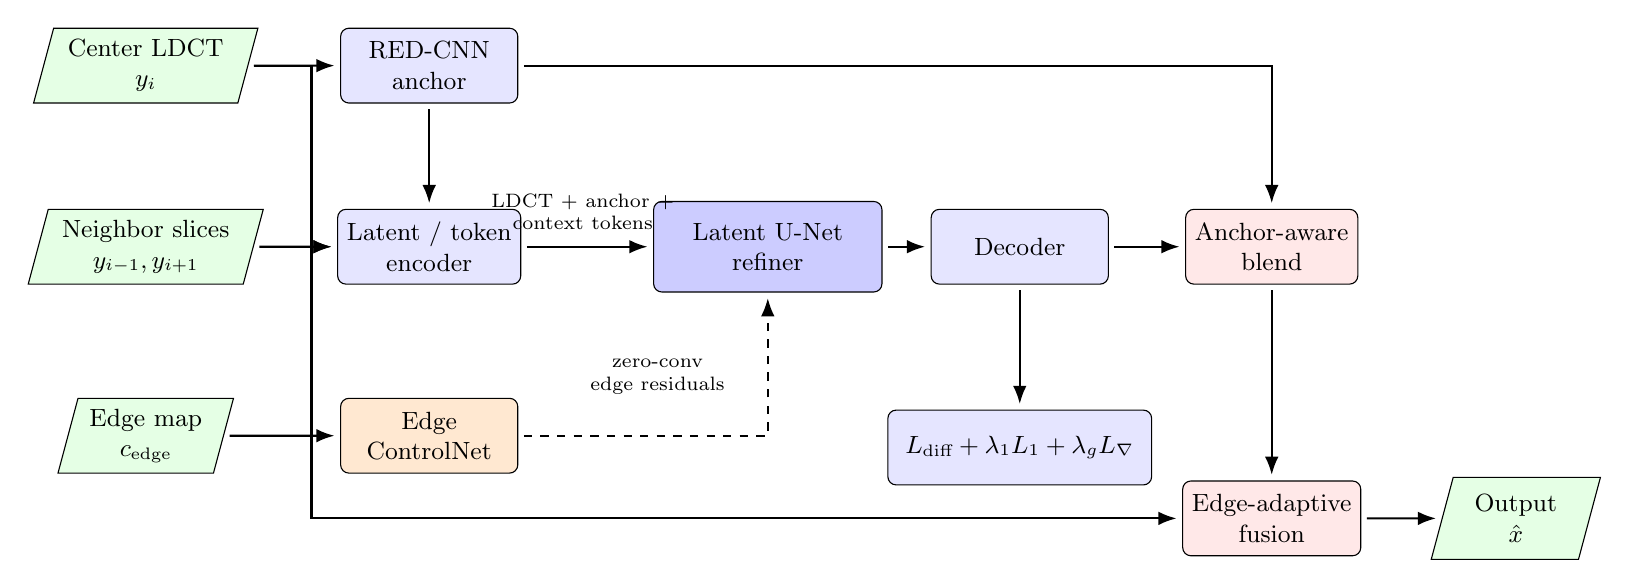
\begin{tikzpicture}[>=Latex, every node/.style={font=\small}]
    \tikzstyle{data}=[trapezium, trapezium left angle=75, trapezium right angle=105, draw, fill=green!10, minimum height=0.95cm, minimum width=2.15cm, align=center]
    \tikzstyle{block}=[rectangle, draw, rounded corners=3pt, fill=blue!10, minimum height=0.95cm, minimum width=2.25cm, align=center]
    \tikzstyle{control}=[rectangle, draw, rounded corners=3pt, fill=orange!18, minimum height=0.95cm, minimum width=2.25cm, align=center]
    \tikzstyle{merge}=[rectangle, draw, rounded corners=3pt, fill=red!9, minimum height=0.95cm, minimum width=2.15cm, align=center]
    \tikzstyle{flow}=[->, thick, shorten >=2pt, shorten <=2pt]
    \tikzstyle{guide}=[->, dashed, thick, shorten >=2pt, shorten <=2pt]

    \node[data] (ldct) at (0.0, 3.7) {Center LDCT\\$y_i$};
    \node[data] (ctx) at (0.0, 1.4) {Neighbor slices\\$y_{i-1}, y_{i+1}$};
    \node[data] (edge) at (0.0, -1.0) {Edge map\\$c_{\text{edge}}$};

    \node[block] (anchor) at (3.6, 3.7) {RED-CNN\\anchor};
    \node[block] (encoder) at (3.6, 1.4) {Latent / token\\encoder};
    \node[control] (ctrl) at (3.6, -1.0) {Edge\\ControlNet};

    \node[block, fill=blue!20, minimum width=2.9cm, minimum height=1.15cm] (unet) at (7.9, 1.4) {Latent U-Net\\refiner};
    \node[block] (dec) at (11.1, 1.4) {Decoder};
    \node[merge] (blend1) at (14.3, 1.4) {Anchor-aware\\blend};
    \node[merge] (blend2) at (14.3, -2.05) {Edge-adaptive\\fusion};
    \node[data] (out) at (17.4, -2.05) {Output\\$\hat{x}$};
    \node[block, minimum width=3.35cm] (losses) at (11.1, -1.15) {$L_{\text{diff}} + \lambda_1L_1 + \lambda_gL_{\nabla}$};

    \coordinate (encbus) at ($(encoder.west)+(-0.6,0)$);
    \coordinate (ctrlapproach) at (unet.south |- ctrl.east);
    \coordinate (anchorbusa) at ($(anchor.east)+(0.8,0)$);
    \coordinate (anchorbusb) at (blend1.north |- anchorbusa);
    \coordinate (ldctbusa) at ($(ldct.east)+(0.8,0)$);
    \coordinate (ldctdrop) at (ldctbusa |- blend2.west);

    \draw[flow] (ldct.east) -- (anchor.west);
    \draw[flow] (ldct.east) -- (ldctbusa) |- (encbus) -- (encoder.west);
    \draw[flow] (ctx.east) -- (encbus) -- (encoder.west);
    \draw[flow] (edge.east) -- (ctrl.west);
    \draw[flow] (anchor.south) -- (encoder.north);

    \draw[flow] (encoder.east) -- (unet.west);
    \draw[guide] (ctrl.east) -- (ctrlapproach) -- (unet.south);
    \draw[flow] (unet.east) -- (dec.west);
    \draw[flow] (dec.east) -- (blend1.west);
    \draw[flow] (anchor.east) -- (anchorbusa) -- (anchorbusb) -- (blend1.north);
    \draw[flow] (blend1.south) -- (blend2.north);
    \draw[flow] (ldct.east) -- (ldctbusa) -- (ldctdrop) -- (blend2.west);
    \draw[flow] (blend2.east) -- (out.west);
    \draw[flow] (dec.south) -- (losses.north);

    \node[font=\scriptsize, align=center] at (5.55, 1.84) {LDCT + anchor +\\context tokens};
    \node[font=\scriptsize, align=center] at (6.5, -0.25) {zero-conv\\edge residuals};
\end{tikzpicture}
}
\caption{Overview of the proposed \hybrid{}. A RED-CNN anchor provides strong pixel fidelity, neighboring slices supply 2.5D context, and an edge-guided ControlNet injects structural residuals into the latent diffusion backbone. During training, decoded predictions receive auxiliary intensity and gradient losses. During inference, the diffusion output is first blended conservatively with the RED-CNN anchor and then re-grounded to the observed LDCT slice through edge-adaptive fusion.}
\label{fig:arch}
\end{figure*}

\subsection{Anchor-Aware Inference with Edge-Adaptive Fusion}
The final reported model uses a tuned direct-$x_0$ inference path rather than default multi-step img2img sampling. We found that a single-step latent estimate at a moderate diffusion timestep was more stable for the current prototype:
\begin{equation}
    \hat{z}_0 =
    \frac{z_t - \sqrt{1-\bar{\alpha}_t}\,\epsilon_{\theta}(z_t,t,\mathcal{C})}
    {\sqrt{\bar{\alpha}_t}},
\end{equation}
with direct timestep $t=20$ and control conditioning scale $0.8$ selected on the validation set. The decoded prediction $\tilde{x} = \mathcal{D}(\hat{z}_0)$ is not used directly. Instead, we first blend it with the RED-CNN anchor:
\begin{align}
    \bar{x} &= \beta \tilde{x} + (1-\beta) a, \\
    w(u,v) &= \mathrm{clip}\!\left(\alpha - \gamma E(y)_{u,v}, 0, 1\right), \\
    \hat{x}_{u,v} &= w(u,v)\,\bar{x}_{u,v} + \left(1-w(u,v)\right) y_{u,v},
\end{align}
where $E(y)$ is a normalized Sobel-gradient magnitude map. Validation sweeps selected $\beta = 0.03$, $\alpha = 1.0$, and $\gamma = 0.15$. These numbers are informative: the best operating point assigns only a small global weight to the diffusion correction, but that correction is still valuable when it is targeted and structurally guided. In other words, the diffusion branch is most effective here as a conservative anatomical refiner around a strong deterministic backbone, not as a wholesale replacement for it.

\subsection{Conservative Reconstruction Interpretation}
The full method should therefore be read as a measurement-grounded hybrid rather than a free-form generator. RED-CNN provides the high-fidelity anchor. The latent diffusion branch contributes structured residual corrections informed by LDCT appearance, neighboring-slice context, and explicit edges. The final edge-adaptive fusion reintroduces more of the observed LDCT signal where gradients are strong. This layered conservatism is intentional: it reduces the burden on diffusion to hallucinate detail, preserves boundary trustworthiness, and converts the structural advantages of edge guidance into a regime that can compete directly with pixel-optimized deterministic denoisers.

\section{Experimental Setup}
\subsection{Leakage-Free LIDC-IDRI Protocol}
We start from raw LIDC-IDRI DICOM studies~\cite{armato2011}. The public release contains real thoracic CT anatomy but not paired standard-dose/low-dose acquisitions, so we formulate a paired denoising benchmark by corrupting preprocessed clean slices with signal-dependent Gaussian noise. This design preserves real anatomy while maintaining pixel-aligned targets for quantitative evaluation.

Data curation is strict. We scan 382{,}009 candidate DICOM files, keep CT series only, remove 27{,}911 non-CT files, remove 110{,}141 duplicate SOP instance UIDs, and verify finite HU conversion for all retained slices. The final index contains 243{,}957 valid slices from 1{,}010 patients and 1{,}018 series. Splits are assigned at the patient level and persisted to disk, which prevents near-neighbor slices from the same study from leaking across train and test. The resulting patient-level split statistics are summarized in Table~\ref{tab:split}.

\begin{table}[t]
\centering
\small
\caption{Leakage-free patient-level split derived from raw LIDC-IDRI DICOM.}
\label{tab:split}
\begin{tabular}{lccc}
\toprule
Split & Patients & Series & Slices \\
\midrule
Train & 808 & 814 & 191{,}319 \\
Validation & 101 & 101 & 24{,}939 \\
Test & 101 & 103 & 27{,}699 \\
\bottomrule
\end{tabular}
\end{table}

To keep the study reproducible on a single RTX 5080 workstation while still operating on real DICOM anatomy, the reported diffusion experiments use a fixed medium-scale protocol sampled from this split: 4{,}096 training slices and 256 evaluation slices per split. RED-CNN is trained on the same patient-level slice budget for direct comparison.

\subsection{Preprocessing and Models}
All slices are clipped to $[-1000, 1000]$ HU, normalized to $[-1,1]$, and resized to $256 \times 256$. The synthetic low-dose corruption follows the repository's signal-dependent Gaussian model with noise range $[0.01, 0.06]$ and coefficient $0.02$.

The final \hybrid{} combines three trained components under one inference pipeline. The first is a RED-CNN anchor model with 5 convolutional and 5 deconvolutional stages, base width 96, and a mixed reconstruction objective; it is trained for 6 epochs under the patient-level medium-scale subset. The second is an edge-guided latent diffusion refiner with a $32 \times 32 \times 4$ latent representation, a trainable tiny U-Net, and a ControlNet branch with one-channel edge conditioning. The third is a lightweight conditioning pathway that encodes the immediate previous and next slices, giving the diffusion branch 2.5D context without moving to full 3D training.

Stable mixed-precision training required BF16 on the RTX 5080. The final hybrid diffusion model trains for 4 epochs with learning rate $8\times 10^{-5}$, anchor-conditioning dropout 0.1, neighboring-slice count 1, and auxiliary reconstruction weights $\lambda_1=0.5$ and $\lambda_g=0.1$. The matched no-edge ablation uses the same diffusion configuration but zeros the edge input during both training and evaluation. We also implemented a stronger pretrained latent-backbone path, but under the same medium-scale budget the most reliable improvement came from hybrid refinement around the RED-CNN anchor rather than from swapping in a larger latent prior.

\subsection{Fast Ordinary Baselines}
To provide additional context without long retraining cycles, we also evaluate ordinary nonlearned denoisers directly on the saved validation and test arrays. These experiments require no model training and complete in well under one minute on CPU for the full reported sweep. We include Gaussian, median, bilateral, Wiener, and total-variation filters as fast classical references, plus two intentionally simple aggressive smoothers (Gaussian $\sigma=2.0$ and box blur $7 \times 7$) as low-capacity over-smoothing references. This gives a practical view of where the current diffusion prototype sits relative to both naive smoothing and stronger classical denoising behavior under the same synthetic corruption model.

\subsection{Metrics}
We report PSNR, SSIM~\cite{wang2004ssim}, and RMSE on paired clean targets. Because the benchmark is slice-paired and pixel-aligned, these metrics provide a direct view of both numerical fidelity and structural preservation. We also report deltas relative to the raw noisy LDCT baseline.

\section{Results}
\subsection{Main Comparison on the Real Test Protocol}
Table~\ref{tab:main-results} summarizes the main test-set comparison. Four patterns are most important. First, raw edge-guided diffusion alone is not enough to match the strongest deterministic baseline, even though it improves over raw LDCT and over a matched no-edge ablation. Second, RED-CNN remains an extremely strong anchor under this paired synthetic protocol. Third, once diffusion is recast as a refinement module around that anchor and is given 2.5D context plus direct reconstruction supervision, the hybrid system closes the remaining fidelity gap. Fourth, the improvement over RED-CNN is small but consistent across all three reported metrics, which is exactly the regime in which a conservative refinement module should be judged.

\begin{table}[t]
\centering
\small
\caption{Main test-set results on real LIDC-IDRI anatomy with synthetic low-dose corruption. Delta values are measured relative to raw LDCT.}
\label{tab:main-results}
\resizebox{\linewidth}{!}{
\begin{tabular}{lcccccc}
\toprule
Method & PSNR $\uparrow$ & SSIM $\uparrow$ & RMSE $\downarrow$ & $\Delta$PSNR & $\Delta$SSIM & $\Delta$RMSE \\
\midrule
LDCT & 28.2181 & 0.6244 & 0.08176 & 0.0000 & 0.0000 & 0.00000 \\
RED-CNN & 35.0199 & 0.9028 & 0.03598 & +6.8018 & +0.2784 & -0.04577 \\
No-Edge \method{} & 27.6809 & 0.7063 & 0.08328 & -0.5372 & +0.0819 & +0.00152 \\
Edge-Guided \method{} + tuned inference & 28.4629 & 0.7102 & 0.07652 & +0.2447 & +0.0858 & -0.00524 \\
\textbf{\hybrid{} (ours)} & \textbf{35.1197} & \textbf{0.9040} & \textbf{0.03558} & \textbf{+6.9016} & \textbf{+0.2796} & \textbf{-0.04617} \\
\bottomrule
\end{tabular}
}
\end{table}

\subsection{Fast Classical Context}
Figure~\ref{fig:overview} adds a visual metric-by-metric summary. Aggressive smoothers such as Gaussian $\sigma=2.0$ remain below the diffusion-family refiners, while stronger classical filters such as TV denoising remain competitive under the present signal-dependent Gaussian corruption. This is useful because it shows that the benchmark does not automatically favor learned generative models and that the hybrid gain is not reducible to trivial smoothing.

\begin{figure*}[t]
\centering
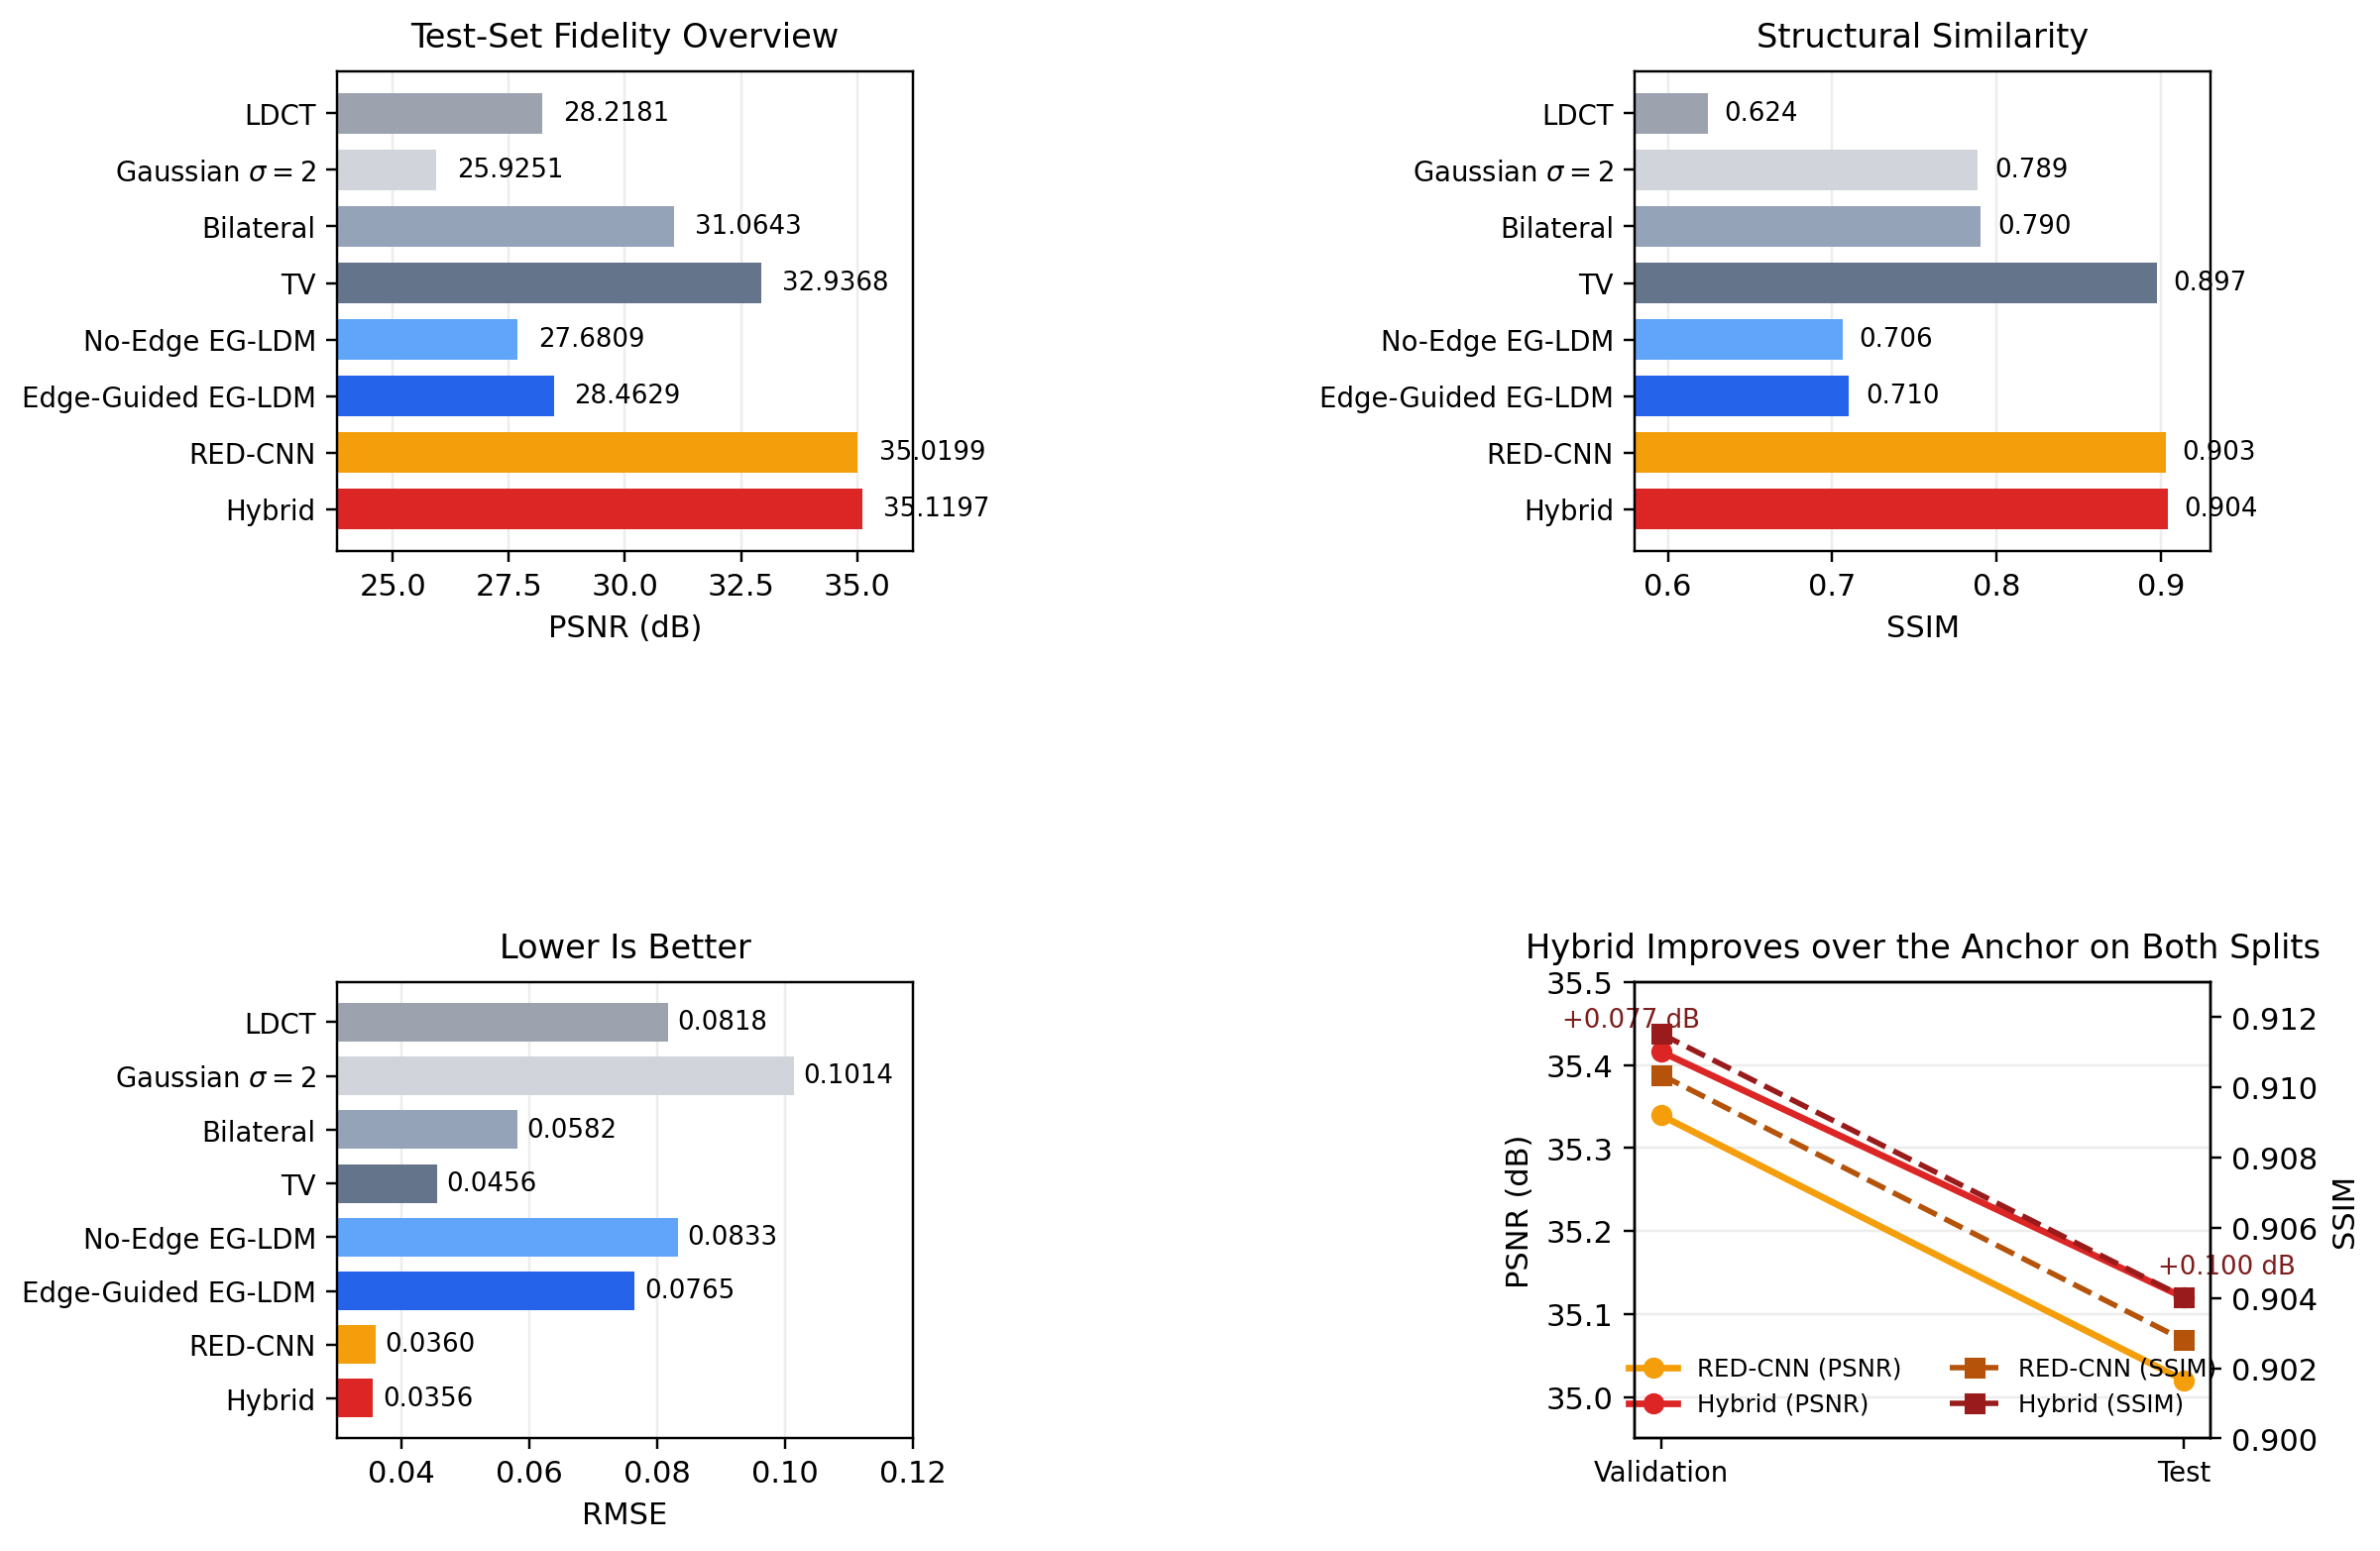
\includegraphics[width=0.94\textwidth]{figures/performance_overview.png}
\caption{Quantitative overview of the real test protocol. The three bar charts compare representative classical, diffusion, and hybrid methods across PSNR, SSIM, and RMSE. The line chart shows that the final hybrid refiner improves consistently over the RED-CNN anchor on both validation and test splits.}
\label{fig:overview}
\end{figure*}

\begin{figure}[t]
\centering
\begin{subfigure}[t]{0.98\linewidth}
    \centering
    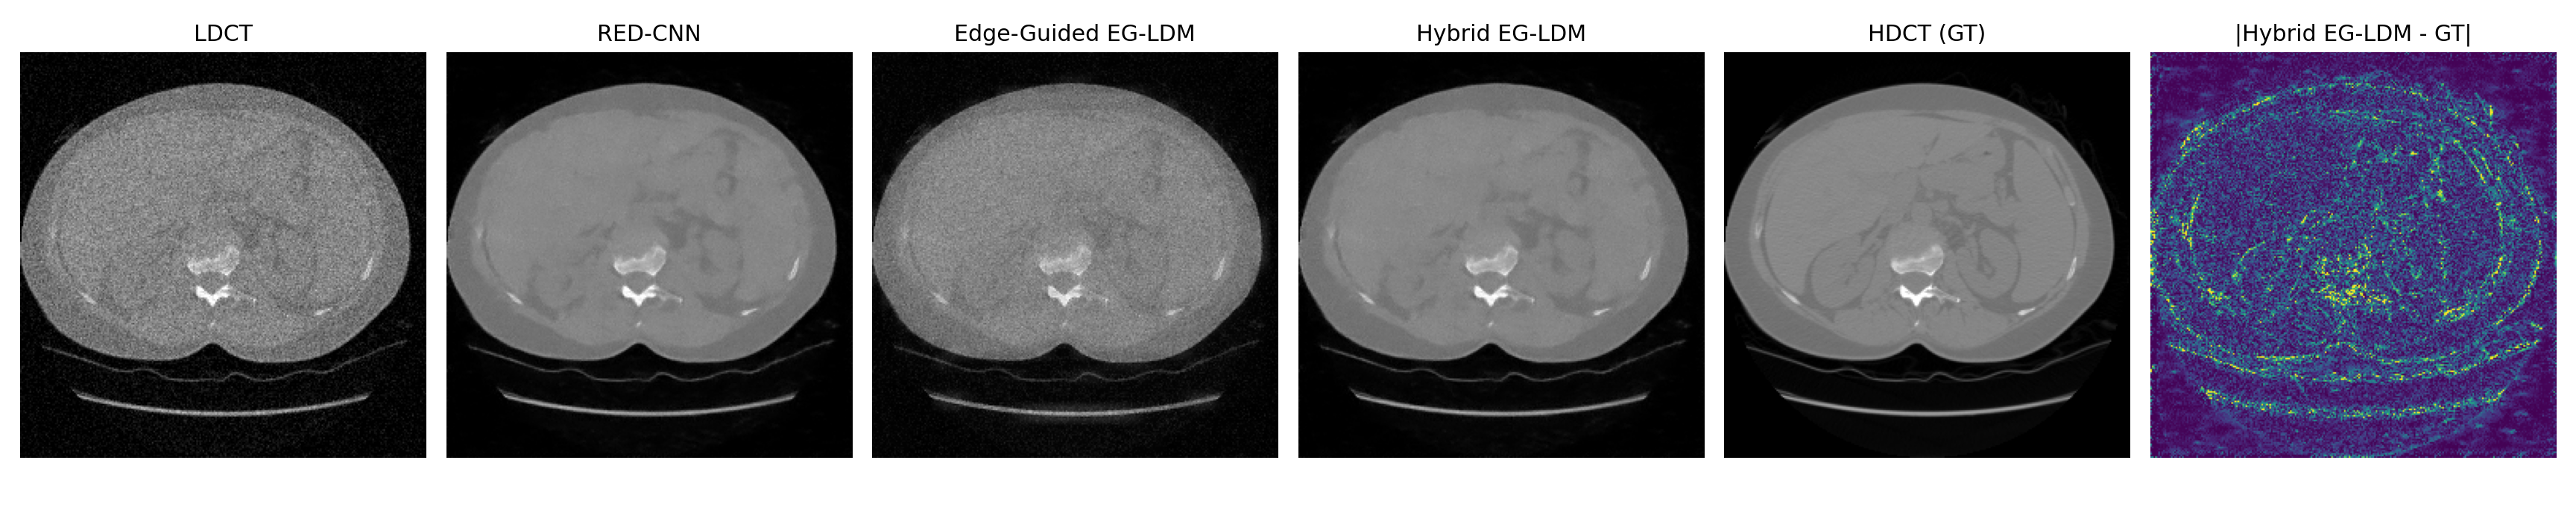
\includegraphics[width=\linewidth]{figures/hybrid_comparison.png}
    \caption{Representative slice-level comparison for \hybrid{}; the rightmost panel is a pseudocolor absolute-error heatmap rather than a CT intensity image.}
\end{subfigure}

\vspace{0.4em}

\begin{subfigure}[t]{0.98\linewidth}
    \centering
    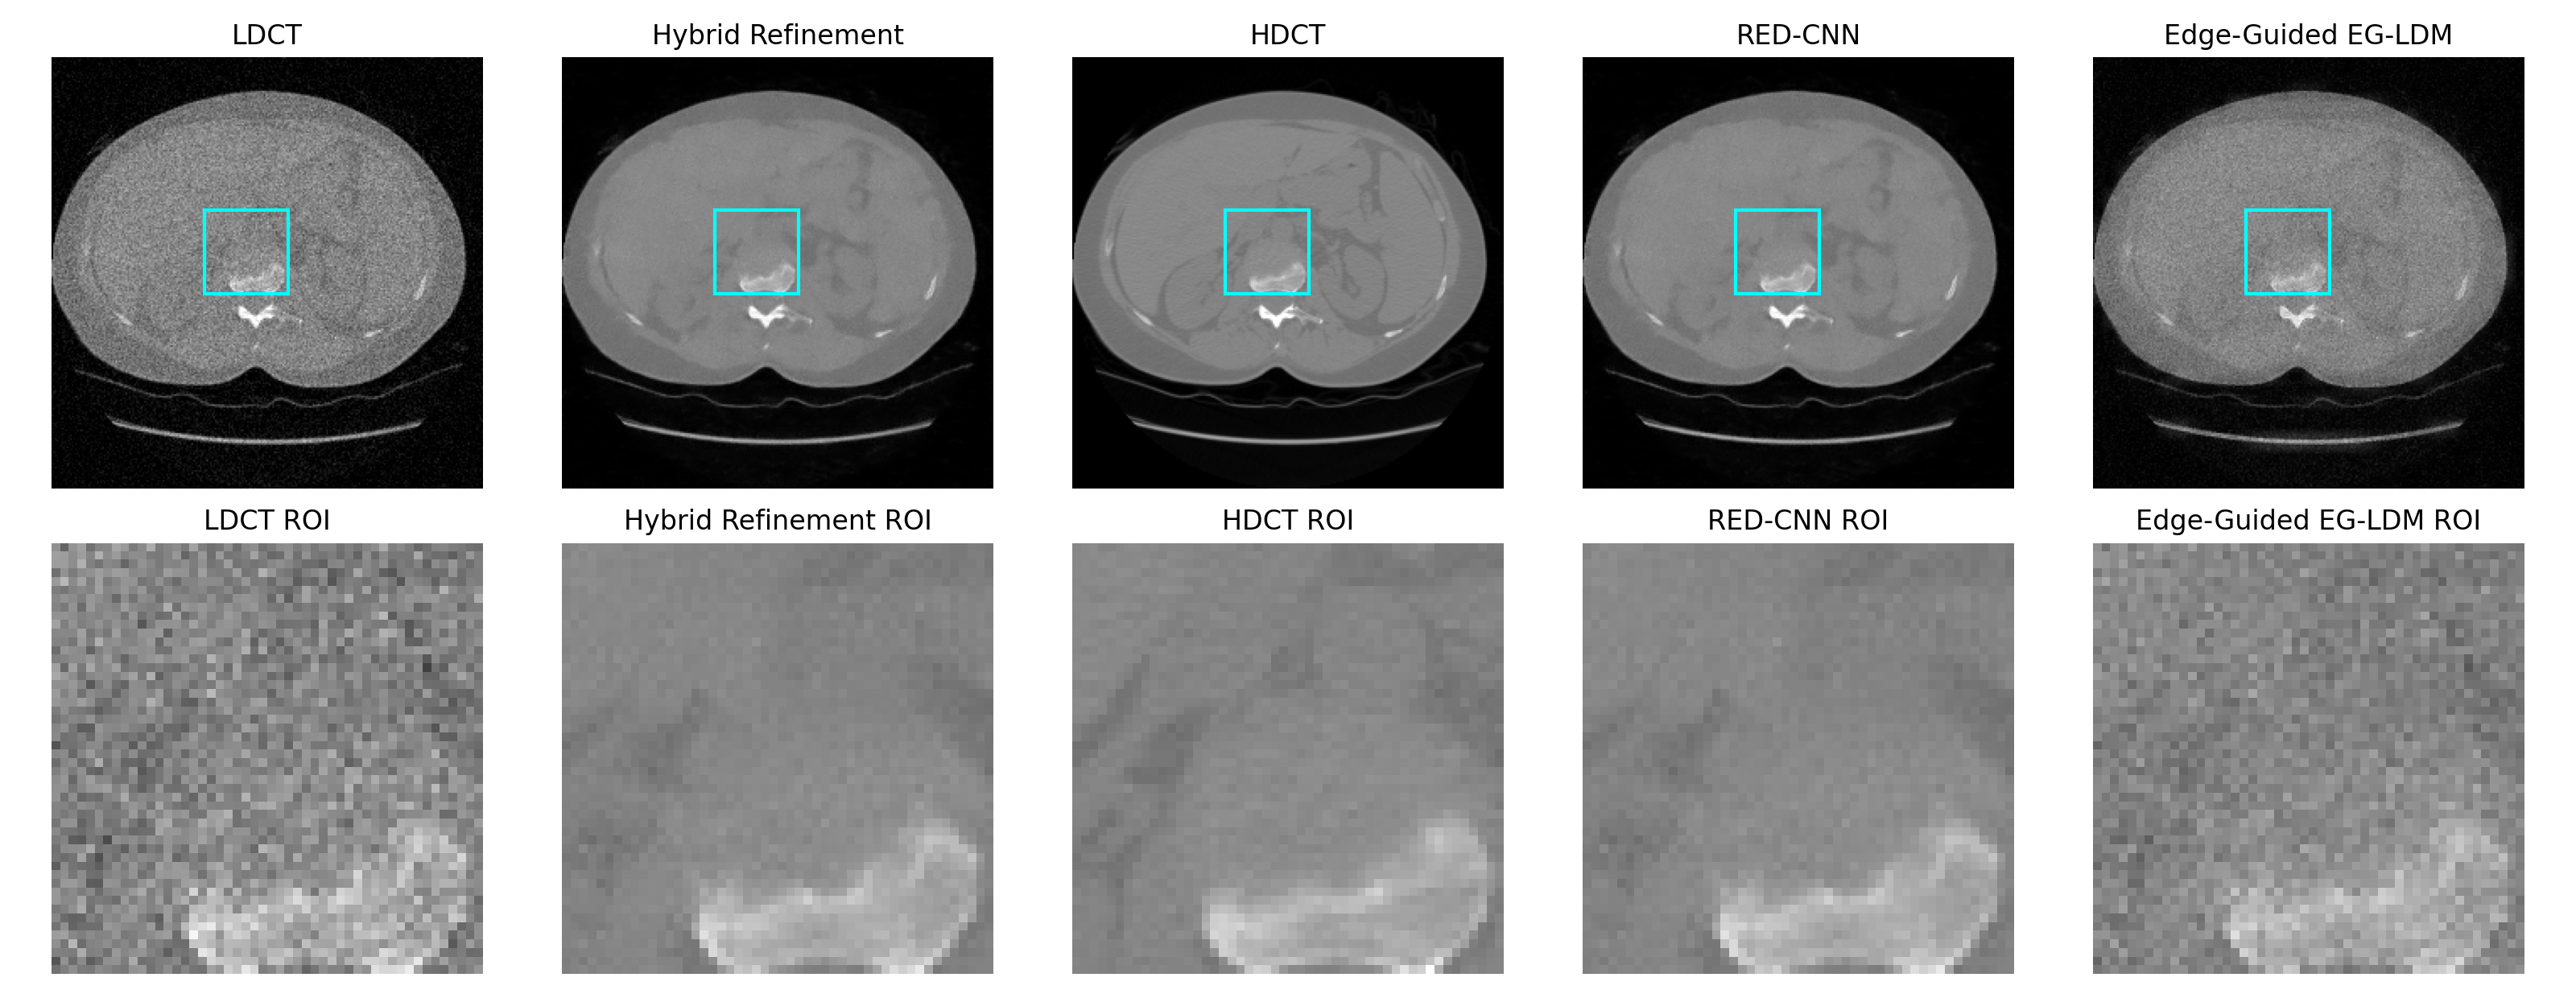
\includegraphics[width=\linewidth]{figures/hybrid_roi.png}
    \caption{ROI zoom emphasizing the vertebral boundary and adjacent soft tissue detail.}
\end{subfigure}
\caption{Qualitative results on the real test protocol. In the comparison panels, HDCT denotes the clean preprocessed LIDC slice used as the synthetic target, not a separately acquired paired high-dose scan. The standalone edge-guided diffusion model improves over LDCT but remains softer than RED-CNN. The proposed \hybrid{} preserves the anchor's sharpness while reducing residual local error, which is consistent with its small but measurable quantitative gain over RED-CNN.}
\label{fig:qualitative}
\end{figure}

\subsection{Ablation: From Edge Guidance to Hybrid Refinement}
The final ablation asks whether diffusion refinement still helps once the strong RED-CNN anchor is already in place. The answer is yes, but in a deliberately modest regime. On validation, \hybrid{} improves over the anchor from 35.3394 to 35.4163 dB PSNR and from 0.9104 to 0.9115 SSIM while reducing RMSE from 0.03478 to 0.03447. On test, the same trend persists: PSNR increases from 35.0199 to 35.1197, SSIM from 0.9028 to 0.9040, and RMSE decreases from 0.03598 to 0.03558. The right panel of Fig.~\ref{fig:overview} visualizes this split-wise consistency. Together with the no-edge versus edge-guided gap already visible in Table~\ref{tab:main-results}, this yields a coherent two-stage conclusion: edge guidance improves the diffusion family, and anchor-conditioned hybridization translates that structural gain into slightly better final fidelity than the deterministic anchor alone.

\section{Discussion}
The experiments support three conclusions. First, patient-level curation is a prerequisite for credible evidence in medical-image restoration; once slice leakage is removed and HU conversion is verified, the benchmark becomes substantially more meaningful. Second, explicit edge guidance improves the diffusion family in a repeatable way even though the edge map is extracted from noisy LDCT itself. Third, the best role for diffusion in this medium-scale paired setting is hybrid and conservative: RED-CNN supplies the high-fidelity anchor, while edge-guided diffusion contributes a smaller residual correction that slightly but consistently improves the final result.

The broader interpretation is methodological. The study shows where gains arise: from leakage-free evaluation, from edge-aware conditioning, from 2.5D anatomical context, from direct reconstruction regularization, and from inference rules that keep the result tethered to both the RED-CNN anchor and the observed LDCT slice. These design elements remain reusable even if future work swaps in a stronger latent backbone or a more realistic scanner-noise model.

\section{Broader Impact}
Improved LDCT denoising could reduce radiation burden by making lower-dose acquisitions more usable in screening and follow-up settings. The main caution is that generative restoration should be treated as assistive rather than autonomous. Structural control and conservative residual fusion are practical safeguards, but clinical deployment still requires reader studies, uncertainty analysis, and scanner-to-scanner validation.

\section{Conclusion}
We presented a leakage-free real-data study of low-dose CT denoising on raw LIDC-IDRI DICOM and used it to trace a full design progression: from standalone latent diffusion, to edge-guided diffusion, to a hybrid diffusion-refinement pipeline anchored by RED-CNN. The resulting benchmark uses verified HU conversion, persisted patient-level splits, real DICOM anatomy, synthetic low-dose corruption, and matched baselines spanning LDCT, fast classical filters, deterministic CNN denoising, and diffusion-family ablations.

Empirically, two findings are clear. Edge guidance materially improves the diffusion family over a matched no-edge ablation, and the strongest use of diffusion here is hybrid rather than standalone: conditioned on a RED-CNN anchor, neighboring slices, and explicit edges, and trained with direct reconstruction regularization plus conservative inference fusion, diffusion refinement reaches PSNR 35.12, SSIM 0.9040, and RMSE 0.03558 on the real test protocol, slightly exceeding the standalone RED-CNN baseline. The practical conclusion is that, for medical restoration tasks where hallucination control and pixel fidelity both matter, diffusion is most compelling as a structurally informed refinement mechanism around a strong deterministic estimate.

\clearpage
{\small
\begin{thebibliography}{99}
\setlength{\itemsep}{0.1em}

\bibitem{brenner2007}
Brenner, D. J., and Hall, E. J. (2007).
Computed tomography --- an increasing source of radiation exposure.
\textit{New England Journal of Medicine}, 357(22), 2277--2284.

\bibitem{armato2011}
Armato, S. G., McLennan, G., Bidaut, L., McNitt-Gray, M. F., Meyer, C. R., Reeves, A. P., et al. (2011).
The lung image database consortium (LIDC) and image database resource initiative (IDRI): A completed reference database of lung nodules on CT scans.
\textit{Medical Physics}, 38(2), 915--931.

\bibitem{buades2011}
Buades, A., Coll, B., and Morel, J.-M. (2011).
Non-local means denoising.
\textit{Image Processing On Line}, 1, 208--212.

\bibitem{dabov2007}
Dabov, K., Foi, A., Katkovnik, V., and Egiazarian, K. (2007).
Image denoising by sparse 3-D transform-domain collaborative filtering.
\textit{IEEE Transactions on Image Processing}, 16(8), 2080--2095.

\bibitem{ronneberger2015}
Ronneberger, O., Fischer, P., and Brox, T. (2015).
U-Net: Convolutional networks for biomedical image segmentation.
\textit{Medical Image Computing and Computer-Assisted Intervention (MICCAI)}, 234--241.

\bibitem{zhang2017dncnn}
Zhang, K., Zuo, W., Chen, Y., Meng, D., and Zhang, L. (2017).
Beyond a Gaussian denoiser: Residual learning of deep CNN for image denoising.
\textit{IEEE Transactions on Image Processing}, 26(7), 3142--3155.

\bibitem{chen2017}
Chen, H., Zhang, Y., Kalra, M. K., Lin, F., Chen, Y., Liao, P., Zhou, J., and Wang, G. (2017).
Low-dose CT with a residual encoder-decoder convolutional neural network.
\textit{IEEE Transactions on Medical Imaging}, 36(12), 2524--2535.

\bibitem{yang2018}
Yang, Q., Yan, P., Zhang, Y., Yu, H., Shi, Y., Mou, X., Kalra, M. K., Zhang, Y., Sun, L., and Wang, G. (2018).
Low-dose CT image denoising using a generative adversarial network with Wasserstein distance and perceptual loss.
\textit{IEEE Transactions on Medical Imaging}, 37(6), 1348--1357.

\bibitem{yi2018}
Yi, X., and Babyn, P. (2018).
Sharpness-aware low-dose CT denoising using conditional generative adversarial network.
\textit{Journal of Digital Imaging}, 31(5), 655--669.

\bibitem{you2018}
You, C., Li, G., Zhang, Y., Zhang, X., Shan, H., Li, M., Ju, S., Zhao, Z., Zhang, Z., Cong, W., Vannier, M. W., and Wang, G. (2018).
Structurally-sensitive multi-scale deep neural network for low-dose CT denoising.
\textit{IEEE Access}, 6, 41839--41855.

\bibitem{wang2004ssim}
Wang, Z., Bovik, A. C., Sheikh, H. R., and Simoncelli, E. P. (2004).
Image quality assessment: From error visibility to structural similarity.
\textit{IEEE Transactions on Image Processing}, 13(4), 600--612.

\bibitem{sohldickstein2015}
Sohl-Dickstein, J., Weiss, E., Maheswaranathan, N., and Ganguli, S. (2015).
Deep unsupervised learning using nonequilibrium thermodynamics.
\textit{International Conference on Machine Learning}, 2256--2265.

\bibitem{ho2020}
Ho, J., Jain, A., and Abbeel, P. (2020).
Denoising diffusion probabilistic models.
\textit{Advances in Neural Information Processing Systems}, 33, 6840--6851.

\bibitem{song2021sde}
Song, Y., Sohl-Dickstein, J., Kingma, D. P., Kumar, A., Ermon, S., and Poole, B. (2021).
Score-based generative modeling through stochastic differential equations.
\textit{International Conference on Learning Representations}.

\bibitem{song2021ddim}
Song, J., Meng, C., and Ermon, S. (2021).
Denoising diffusion implicit models.
\textit{International Conference on Learning Representations}.

\bibitem{nichol2021}
Nichol, A. Q., and Dhariwal, P. (2021).
Improved denoising diffusion probabilistic models.
\textit{International Conference on Machine Learning}, 8162--8171.

\bibitem{saharia2021}
Saharia, C., Fleet, D. J., Ho, J., Norouzi, M., Salimans, T., and Chan, W. (2021).
Image super-resolution via iterative refinement.
\textit{IEEE/CVF International Conference on Computer Vision}, 1543--1552.

\bibitem{chung2022}
Chung, H., Kim, J., Mardani, M., Delbracio, M., Choi, H., and Ye, J. C. (2022).
Score-based diffusion models for accelerated MRI.
\textit{Medical Image Analysis}, 80, 102479.

\bibitem{rombach2022}
Rombach, R., Blattmann, A., Lorenz, D., Esser, P., and Ommer, B. (2022).
High-resolution image synthesis with latent diffusion models.
\textit{Proceedings of the IEEE/CVF Conference on Computer Vision and Pattern Recognition}, 10684--10695.

\bibitem{zhang2023controlnet}
Zhang, L., Rao, A., and Agrawala, M. (2023).
Adding conditional control to text-to-image diffusion models.
\textit{Proceedings of the IEEE/CVF International Conference on Computer Vision}, 3836--3847.

\end{thebibliography}
}

\end{document}
